% !TEX root = ./paper.tex
\label{sec:content}

In this section, we describe our \tcpls implementation.  In a nutshell, our implementation offers the following benefits:
($i$) The support of parallel streams and multiplexing over \tcp connections
  with different cryptographic context.
($ii$) An experimental API that wraps \tls and \tcp and enables applications to
    handle multihoming, multipathing, and various transport layer mechanisms.
($iii$) An improved \tcp extensibility mechanism that sends \tcp options
   through the secure \tcpls channel (as described in
   Sec.~\ref{sec:background-design}). We currently support Linux's \tcp User Timeout
   option. Supporting another \tcp option is only a matter of extending the
   sender's API and processing the option on the receiver side. \tcpls's
   internal machinery can already send any \tcp option during (server-side) or
   after (client-side) the handshake.
($iv$) Different multipath modes for the \tcpls streams: bandwidth aggregation or
none.
($v$) The ability for the server to send eBPF bytecode over the secure
  channel to upgrade the client's \tcp congestion control scheme or
  tune other \tcp mechanisms~\cite{brakmo2017tcp, tran2019beyond}.
  Variable-length options (e.g., eBPF bytecode) can be sent within streams to
  take advantage of bandwidth aggregation or Failover if those features are
  used.
($vi$) Different Connection Migration modes: Failover and Application-level
Connection Migration.


\fr{I don't want to give the impression that everything works like a charm -- I
would need 1 more year to have something production ready}
We stress that all of these features have been tested but this prototype is a
research-level implementation. The implementation can
showcase those features but is however not yet ready for production, as many
bugs likely remain despite our unit tests and integration tests. Portability was
neither part of our goals, but might be necessary for a production ready \tcpls
library.  \subsection{The \tcpls API}

The API that applications use to interact with a protocol plays an important
role in enabling them to leverage all the protocol features. The most
popular API to interact with the transport layer remains the BSD socket
API. Researchers and the IETF have explored new ways to expose a transport API~\cite{draft-ietf-taps-arch,hruby2014sockets,rfc6458,hesmans2016enhanced,schmidt2013socket}.

In this spirit, application-level developers would only be required to
configure a \tcpls context and register function callbacks.
%We design \tcpls such
%that the application-level developers can ignore any notion of Network IPC as
%defined by, for example, the POSIX API, the Berkeley socket API or Winsock,
%facilitating application-level development by offering a more concrete
%session-level interface based on asynchronous network events.
%The overall idea is to offer to application developers the opportunity to tune
%the transport protocol for a better usage of the network from their own
%application protocol, which might depend on its distinguishing
%features.
%\todo{we need to explain the mpjoin}
To illustrate \tcpls API's flexibility, we consider a simple
use case inspired by Happy Eyeballs~\cite{rfc8305}. This technique is
used by web browsers when interacting with dual-stack servers. They
try to establish \tcp connections using IPv4 and IPv6 and prefer the
one that offers the lowest latency. This avoids problems when an address
family is broken on a path but not the other and sometimes results in
lower latency~\cite{bajpai2019longitudinal}.

\begin{figure}[!t]
  \resizebox{0.49\textwidth}{!}{%
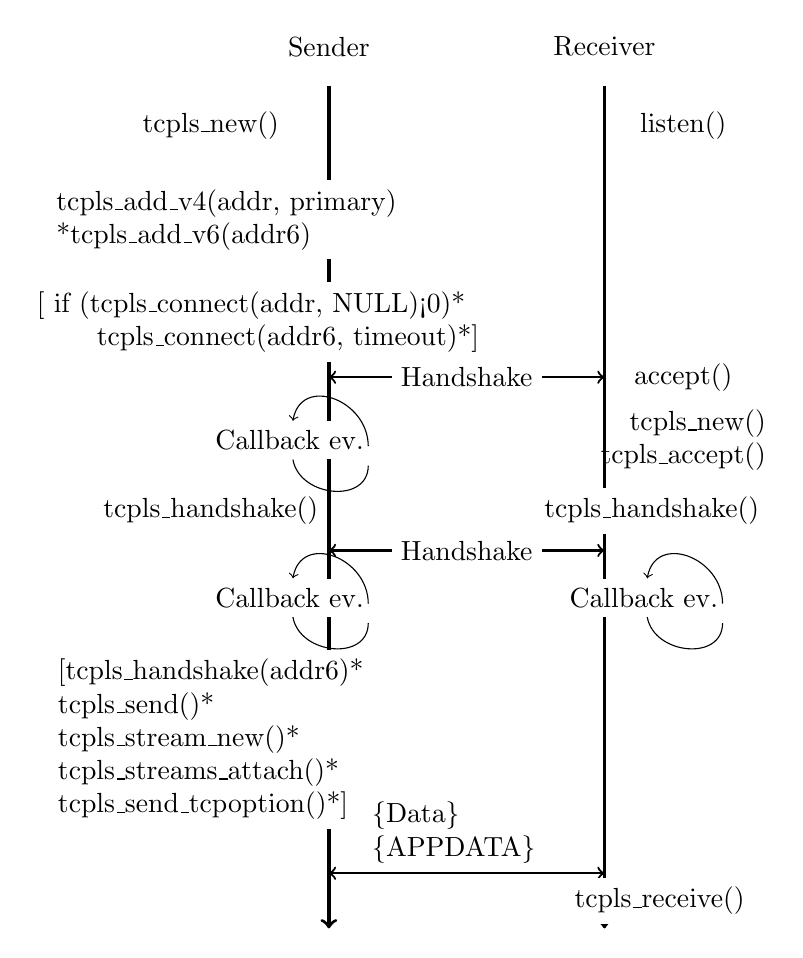
\begin{tikzpicture}
   \colorlet{lightgray}{black!20}
   \tikzstyle{arrow} = [thick,->,>=stealth]
   \tikzset{state/.style={rectangle, dashed, draw, fill=white} }
   \node[black, fill=white] at (0.5,10) {Sender};
   \node[black, fill=white] at (4,10) {Receiver};
   \draw[very thick,->] (0.5,9.5) -- (0.5,-1.2);
   \draw[very thick,->] (4,9.5) -- (4,-1.2);
   \node at (-1,9) {tcpls\_new()};
   \node at (5, 9) {listen()};
   \node[align=left, fill=white] at (-0.8,7.8) {tcpls\_add\_v4(addr,
     primary)\\*tcpls\_add\_v6(addr6)};
   \node[fill=white, align=left] at (-0.4,6.5) {[ if (tcpls\_connect(addr,
     NULL)<0)*\\
     \indent~~tcpls\_connect(addr6, timeout)*]};
   \draw[black, thick, <->] (0.5,5.8) -- (4,5.8) node [midway, fill=white] {\tcp Handshake};
   \node[fill=white] at (0,5) (Callback) {Callback ev.};
   \node at (1,4.8) (here) {};
   \draw [->] (Callback) to[out=-80, in=-90,looseness=1.3] (here)
   to[out=90,in=80,looseness=1.5] (Callback);
   \node at (5, 5.8) {accept()};
   \node[align=right] at (5, 5) {tcpls\_new()\\tcpls\_accept()};
   \node at (-1,4.1) {tcpls\_handshake()};
   \node[fill=white] at (4.6,4.1) {tcpls\_handshake()};
   \draw[black, thick, <->] (0.5,3.6) -- (4,3.6) node [midway, fill=white] {\tcpls Handshake};
   \node[fill=white] at (0,3) (CB2) {Callback ev.};
   \node at (1,2.8) (here2) {};
   \draw [->] (CB2) to[out=-80, in=-90,looseness=1.3] (here2)
   to[out=90,in=80,looseness=1.5] (CB2);
   \node[fill=white] at (4.5,3) (CB3) {Callback ev.};
   \node at (5.5,2.8) (here3) {};
   \draw [->] (CB3) to[out=-80, in=-90,looseness=1.3] (here3)
   to[out=90,in=80,looseness=1.5] (CB3);
   \node[fill=white, align=left] at (-1, 1.2)
   {[tcpls\_handshake(addr6)*\\tcpls\_send()*\\tcpls\_stream\_new()*\\tcpls\_streams\_attach()*\\tcpls\_send\_tcpoption()*]};
   \draw[black, thick, <->] (0.5,-0.5) -- (4,-0.5) node [midway, fill=white,
   above, text width=2.4cm]
   {\{\tcpls Data\} \{APPDATA\}};
   \node[fill=white] at (4.7,-0.85) {tcpls\_receive()};
\end{tikzpicture}
}
\caption{API Workflow example. * means optional call, [ ] means optional call flow, and \{ \} means encrypted.}
  \label{fig:api}
\end{figure}

Fig.~\ref{fig:api} shows an example of our current API workflow. The API can
handle explicit multipath techniques such as Happy Eyeball by chaining
\texttt{tcpls\_connect()} with an appropriate timeout of 50ms, as shown in the
Figure. \tcpls lets the application explicitly choose the multipath mesh by
calling several times \texttt{tcpls\_connect(src, dest,timeout)};. The
application may configure callbacks to connection events that would occur within
\tcpls, such as a connection establishment, a stream attachment, a multipath
join, the reception of a \tcp option to tune \tcp, and more. When multiple
streams are attached to multiple \tcp connections, the application may configure
various \tcpls behaviours. Among them, we support HOL-blocking avoidance,
aggregation of bandwidth with multipathing, connection failover, and connection
migration. Note that, HOL-blocking avoidance is incompatible with the
aggregation of bandwidth with multipathing (the application can do either one
but not both at the same time).



%Note, those features are not stable yet, and many bugs remain to be fixed.

\subsection{Multipathing}

\subsubsection{Data Aggregation}
The application can connect and join multiple \tcp connection to
the same \tcpls session. As soon as one of the peers attaches streams to
different \tcp connections of the session, and enables the aggregation mode,
\tcpls adds a sequence number encrypted in the \tls record payload. This
sequence number is used to reorder the received records after decryption. Our
current state of implementation supports one global ordering, but
we envision for the \tcpls protocol to have streams potentially detached from
the global orderings. For example, a HTTP application may want to use an
aggregation mode for 2 streams over 2 \tcp connections downloading a video
content for the video playback engine, but the other streams used by the HTTP
client do not necessarly need to be part of the multipath bandwidth aggregation.
Such a feature may be implemented through a negotiation of the aggregation
mode.

The implementation currently supports a round-robin scheduler. We expect in the
future that the receiver's scheduler might set through the API, or even sent
from the peer to enable an efficient scheduling against particular sending patterns. The more
the \tcpls receives the records in order, the more \tcpls can deliver them in a zero-copy
fashion to the application. When some record number is not the next expected
record, there is a copy of the record content made within a reordering buffer.
\fr{Do I need to discuss the complexity of the algorithms implemented, and some
  particular memory tricks used?}

\subsubsection{Failover}\label{failover}
While Data Aggregation is exposed to the application, in the sense that the
application uses the API to explicitly connect its session through multiple
paths and activate aggregation, Failover is a binary mode fully internal to
\tcpls. Once activated, \tcpls exchanges acknowledgments for records received in
each stream. The acknowldgment is stream-based and configurable. The default
acknowledgment policy sends an ack every 16 received records, or when a
stream has process more than $249,600$ bytes since the last acknowledgment.
When a \tcp connection sustaining \tcpls streams suffers from a network outage
(e.g., a $RST$ is received or the connection became idle for too long), we move
the stream to a new \tcp connection, retransmit the unacked records and resume
the transfer. Our prototype handles failover over v4 or v6 \tcp connection, and
by default, chooses a different source and destination address than the failed
\tcp connection if some are available. Failover might be negotiated by both
party, or enabled by default by both party. Depending on the application type,
Failover might be enabled or not by default and a negotiatiation through \tcpls's
control channel should happen to change its value (on/off).

\subsubsection{Application-level Connection Migration}
\label{sec:connmigr}

Given the availability of multiple IP paths, connection migration might be a
powerful tool to improve the application network's reliability. Applications
can take advantage of the \tcpls API to migrate their traffic from one network
path to another. When an application feels right to migrate its connection, it
can follow those simple steps: activating the multipath aggregation
mode, then making a \tcpls join handshake on the new path. Then, opening a new stream
and attaching it to the new \tcp connection, and closing the initial
stream would make the data transfert enter in a temporary two-paths aggregated mode in
which the other peer's first path flushes its data if any, and then gracefully close the \tcp
connection achieving a smooth migration. In practice, such a migration would
achieve better goodput than a QUIC single-path migration design in which the
data path is temporally broken and then recovered. In our design, the
application can make such a migration in 4 API calls.

\subsection{TCP Options and Kernel extensibility}

\subsection{QUIC-like roundtrips}

One argument for QUIC's usage on the web was a quicker handshake roundtrip.
Compared to TLS/TCP, QUIC has only one handshake and can then proceed with the
application data. $TLS/TCP$ has two: First, the \tcp three-way handshake, and
then the \tls handshake. \tcpls can use \tcp's TFO~\cite{radhakrishnan2011tcp}
and send the \texttt{ClientHello} message within the \tcp SYN's payload,
achieving the same roundtrips than QUIC. However, TFO suffers from privacy
issues~\cite{sy2020enhanced}, thus we did not enabled it by default. In the
future, we may expect to revise our choice if a solution similar to \tcp
FOP~\cite{sy2020enhanced} gets implemented in the Linux kernel.


